
\documentclass[conference]{IEEEtran}

\usepackage{cite}
\usepackage{graphicx}
\usepackage{amsmath}
\usepackage{amssymb}
\usepackage{color}
\usepackage{caption}
%\usepackage{subcaption}
\usepackage{subfig}
\usepackage{multirow}

\graphicspath{{images/}}




% *** Do not adjust lengths that control margins, column widths, etc. ***
% *** Do not use packages that alter fonts (such as pslatex).         ***
% There should be no need to do such things with IEEEtran.cls V1.6 and later.
% (Unless specifically asked to do so by the journal or conference you plan
% to submit to, of course. )


% correct bad hyphenation here
\hyphenation{op-tical net-works semi-conduc-tor}


\begin{document}
%
% paper title
% Titles are generally capitalized except for words such as a, an, and, as,
% at, but, by, for, in, nor, of, on, or, the, to and up, which are usually
% not capitalized unless they are the first or last word of the title.
% Linebreaks \\ can be used within to get better formatting as desired.
% Do not put math or special symbols in the title.
\title{Limits of Deep Learning}


% author names and affiliations
% use a multiple column layout for up to three different
% affiliations
\author{\IEEEauthorblockN{Simon Jenni}
\IEEEauthorblockA{University of Bern\\
simujenni@students.unibe.ch}
\and
\IEEEauthorblockN{Simon Brulhart}
\IEEEauthorblockA{University of Fribourg\\
simon.brulhart@unifr.ch}
}


% make the title area
\maketitle

% As a general rule, do not put math, special symbols or citations
% in the abstract
\begin{abstract}
Current natural language models try to capture semantic and syntactic relationships between words.
This allows them to answer questions in the form of analogies: "X is to Y as U is to ?".
We study the performance of the word2vec tool on this task. To this end, we analyse the sensitivity to different hyperparameter choices.
We generate new question sets and demonstrate the models (in)ability to learn and answer on domain-specific knowledge. 
To offer a more detailed view of the model's performance, we introduce a broader definition of accuracy which is taking into account how far off the model is in a failure case and study how the choice of similarity measure influence the model's accuracy.
To increase the models accuracy on solving analogies, we propose a mean-shift procedure as preliminary step to computing the query vector and a combination of analogy interpretations for solving for the most similar word-vector. The effectiveness  of these approaches are demonstrated on a generalised question set.


\end{abstract}

% no keywords


% For peer review papers, you can put extra information on the cover
% page as needed:
% \ifCLASSOPTIONpeerreview
% \begin{center} \bfseries EDICS Category: 3-BBND \end{center}
% \fi
%
% For peerreview papers, this IEEEtran command inserts a page break and
% creates the second title. It will be ignored for other modes.
\IEEEpeerreviewmaketitle


\section{Introduction}

Recent state-of-the-art natural language models represent words by embedding them
as vectors in a continuous vector space \cite{mikolov2013efficient} \cite{pennington2014glove}.
These embeddings are learned as weights of a recurrent neural network language model.
It has been demonstrated that the distributed representation of words as vectors
in a common vector-space captures not just syntactic similarities (\textit{e.g.} $cat$
is close to $cats$) but semantic similarities as well. Concretely, the model's ability to
perform "word-arithmetic" has been shown in \cite{mikolov2013linguistic}.
To exemplify this, let $f$ be the word-embedding function. Ideally, we would then
have an embedding where distances in vector-space give a measure of
semantic-similarity between the words. For two word pairs such as $(king:man)$
and $(queen:woman)$ which have the same relation (or similarity), we would
obtain $f(king)-f(man) \approx f(queen) - f(woman)$ or equivalently $f(king)-f(man) +
f(woman) \approx f(queen)$. This of course is equivalent to the analogy "$king$ is
to $man$ as $queen$ is to $woman$". 

The goal of this work is to further evaluate the performance
of the popular word2vec tool on these tasks. We evaluate the effect of
different choices for model-architectures and hyperparameters on the performance and test
the limits of the models semantic-analysis capabilities on new challenging test data. 
The ability to learn analogies has  been demonstrated on rather general and 
hand-picked test-sets. We test the models ability to learn domain-specific knowledge by 
generating questions that test relationships such as $Brand \thicksim Country$ 
and $Movie \thicksim Director$. Previous work focuses on the nearest 
resulting vector in the embedding space when evaluating the accuracy of this word-arithmetic. 
We generalise the notion of accuracy by considering not only the nearest word-vector, but 
consider the set of the $k$ nearest vectors and test whether the target word is present therein. 


The content of this paper is structured as follows: Section \ref{sec:relwork} gives an overview 
of relevant previous works. In Section \ref{sec:model} we present a brief overview of the underlying 
model and in Section \ref{sec:exp} we outline the experimental setup and testdata used. 
The results of the experiments are then reported in Section \ref{sec:res} before we conclude
in \ref{sec:end}.


\section{Related Work}
\label{sec:relwork}

The work by Tomas Mikolov \cite{mikolov2013efficient}, where the models were introduced,
reports results on a test set they themselves created. The set contained five types of semantic
questions where relations such as $Country \thicksim Currency$ or $Country \thicksim Capital$
were tested. In \cite{mikolov2013linguistic} the models performance on semantical
similarity has been demonstrated on SemEval-2012 Task 2 \cite{jurgens2012semeval}.
The objective in this task is to decide how similar two target wordpairs such as
$(glass:break)$ and $(soldier:fight)$ are with respect to a relation "an $X$ typically $Y$". 
Though the model is not directly trained on this task, it achieved better results than  the previous
best methods. 

In \cite{levy2015improving} Levy \textit{et. al.} provide a comprehensive study of several word 
embedding techniques on the two tasks \textit{Word Similarity} and \textit{Analogy}. 
They conclude that much of the performance gains of new embedding
methods stem from design choices and parameter optimisation rather than the 
underlying algorithms. Performance estimation was based only on the testdata sets 
introduced in \cite{mikolov2013efficient} and \cite{mikolov2013linguistic}.

In a previous work \cite{levy2014dependency} they show that generalising the Skip-Gram 
model's negative sampling to arbitrary contexts results in the model learning 
functional similarities. They demonstrate this by manually inspecting the top $k$ most 
similar words to a given query word. A query \textit{e.g.} for \textit{Hogwarts} returns
a list of famous schools in their modified Skip-Gram implementation while CBOW returns 
a list of \textit{Harry Potter} characters.

\begin{figure}[t]
\centering
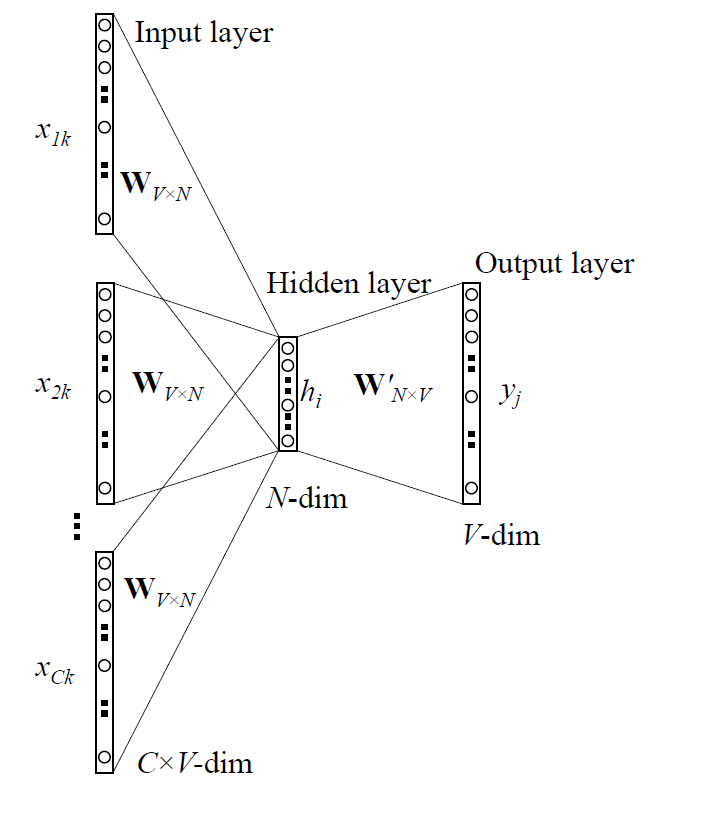
\includegraphics[width=0.375\textwidth]{cbow}
\caption{Architecture of the CBOW model. The three one-hot input vectors represent the context 
of a centre word in a sentence and the output vector is a vector with probabilities over possible 
centre-words. }
\label{fig:cbow}
\end{figure}

\section{The Models of word2vec}
\label{sec:model}

The word2vec tool is an implementation of the Continuous Bag-of-Words (CBOW) and Skip-Gram
models introduced in \cite{mikolov2013efficient}. Both of these models are based
on  two-layer  neural networks with architectures depicted in Figure~\ref{fig:cbow}
and Figure~\ref{fig:skip}. The two architectures reflect the objectives of both models: CBOW
is trained to predict the centre word from its context in a sentence while Skip-Gram tries to predict
the context from its centre. Both architectures take vectors of one-hot encoded words as inputs. Let $x_i$
denote an input-vector corresponding to word $i$ and let the input vocabulary be $V$, 
then the inputs to the model are given by the $|V|$-dimensional vectors:
\begin{equation}
w_{a} = \begin{pmatrix}1 \\ 0 \\ 0 \\ \vdots \\ 0 \end{pmatrix},
w_{abandon} = \begin{pmatrix}0 \\ 1 \\ 0 \\ \vdots \\ 0 \end{pmatrix}, \dots ,
w_{zone} = \begin{pmatrix}0 \\ 0  \\ \vdots \\ 0 \\ 1 \end{pmatrix}
\end{equation}

These one-hot vectors get mapped into a $N$-dimensional vector via the $|V| \times N$ weight matrix
$\boldsymbol{W}$.  The hidden unit then accumulates the sum of these vectors for all input
words in the case of CBOW and consists of only the vector associated with the single input in the 
Skip-Gram model. The output of the model is generated by multiplying the hidden-units by
with a $N \times |V|$ weight matrix $\boldsymbol{W'}$ and applying softmax to the result in order to generate a valid
probability distribution over words in the vocabulary. Concretely, given a sequence of 
training words $w_1, w_2, \dots , w_T$ the hidden-states are computed as
\begin{equation}
	h = \boldsymbol{W}w.
\end{equation}

Given the values of the hidden units, the output can be computed as
\begin{equation}
	y = P_t(\boldsymbol{W'}h)
\end{equation}
with the softmax function $P_t$ of a $N$-dimensional vector $x$ given by 
\begin{equation}
	P_t(x)_i = \frac{e^{x_i}}{\sum_{j=1}^{|V|}{e^{x_j}}},
\end{equation}
for $i \in \{1, \hdots , |V|\}$.
The learnt word representations are then given by the columns of $\boldsymbol{W}$.

The models are learnt in an unsupervised fashion where either the centre-word of
a series of words is predicted from its context (CBOW) or the context is
predicted from the centre word (Skip-Gram). Both models try to maximise the
log-likelihood of their output. Training is done via gradient descent using backpropagation
\cite{rumelhart1988learning}.

At test time when looking for the word most similar to a given word $w$ we solve for 
\begin{equation}
	x = \text{argmax}_{v \in V} d(f(w),f(v))
	\label{eq:sim}
\end{equation}
Where $f$ is the embedding and $d$ is a similarity measure. We therefore search for the 
word in the vocabulary which has the minimal distance in the embedding space. The 
model as proposed by \cite{mikolov2013efficient} chose $d$ to be the cosine similarity, 
but we investigate different choices such as $L^p$-norm or Dice similarity.

\begin{figure}[t]
\centering
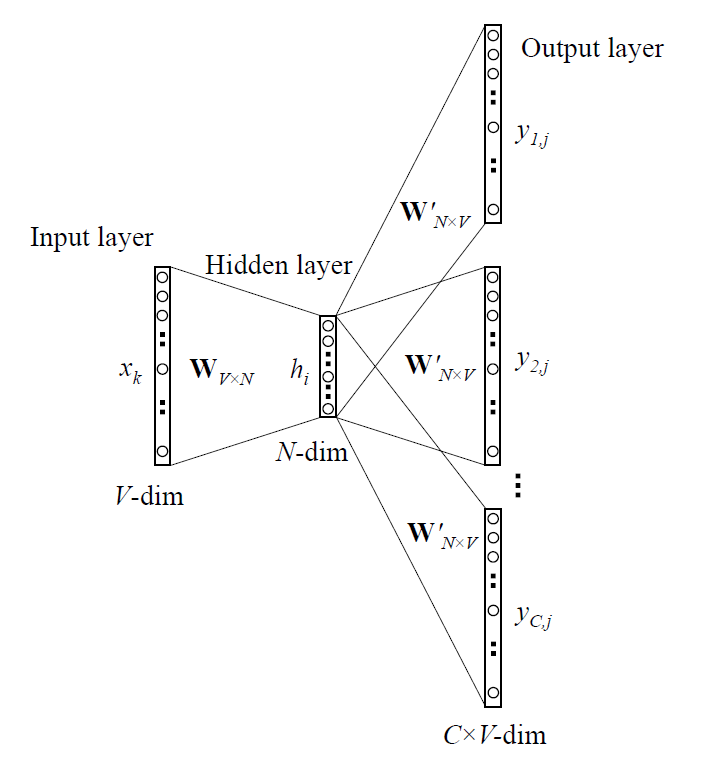
\includegraphics[width=0.4\textwidth]{skip-gram}
\caption{Architecture of the Skip-Gram model. The output of this model are vectors with probabilities 
for the words occurring in the context of the input word.}
\label{fig:skip}
\end{figure}

\subsection{Word Arithmetic for Solving Analogies}
\label{sec:arithm}
Consider the case of an analogy question "$X$ is to $Y$ as $U$ is to $V$" where we are interested in solving for the word $V$. Let $x=f(X)$, $y=f(Y)$ and $u=f(U)$ be the embedded words. The straightforward way of computing $v=f(V)$ is then to use Equation \ref{eq:sim} and solving for 
\begin{equation}
	v = \underset{v \in f(V)}{\text{argmax }}  d(v, u-x+y)
	\label{eq:anal}
\end{equation}

As it turns out however depending on the similarity measure $d(\cdot|\cdot)$ it can be a good idea to consider different approaches such as 
\begin{equation}
	v =  \underset{v \in f(V)}{\text{argmax }}  d(v, u) - d(v, x) + d(v, y)
	\label{eq:anal2}
\end{equation}
The intuition behind this approach is less one of performing word-vector arithmetic and more one of finding the word $V$ most similar to $X$ and $U$ and dissimilar to $Y$. This approach turns out to work considerably better when using the cosine-similarity. Note that  Equations \ref{eq:anal} and  \ref{eq:anal2} are equivalent for 
unit vectors when using the cosine similarity.

\subsection{Considered Similarity Measures}
\label{sec:sim}
In our experiments we considered the following similarity measures:
\begin{equation}
	L^2(x,y) = -||x-y||_2 = -\sqrt{\sum_{i=1}^{n}{(x_i-y_i)^2}}�
\end{equation}
\begin{equation}
	L^1(x,y) = -\sqrt{\sum_{i=1}^{n}{(x_i-y_i)^2}}�
\end{equation}
\begin{equation}
	Dice(x,y) = \frac{xT y}{||x|| + ||y||}
\end{equation}
\begin{equation}
	Cos(x,y) = \frac{x^T y}{||x|| \cdot ||y||}
\end{equation}
We denote the approach in Equation \ref{eq:anal2} with cosine similarity by $cosAdd$ in the results.


\begin{figure*}[t]
\centering
\subfloat[Nearby points in the right are difficult to discriminate]{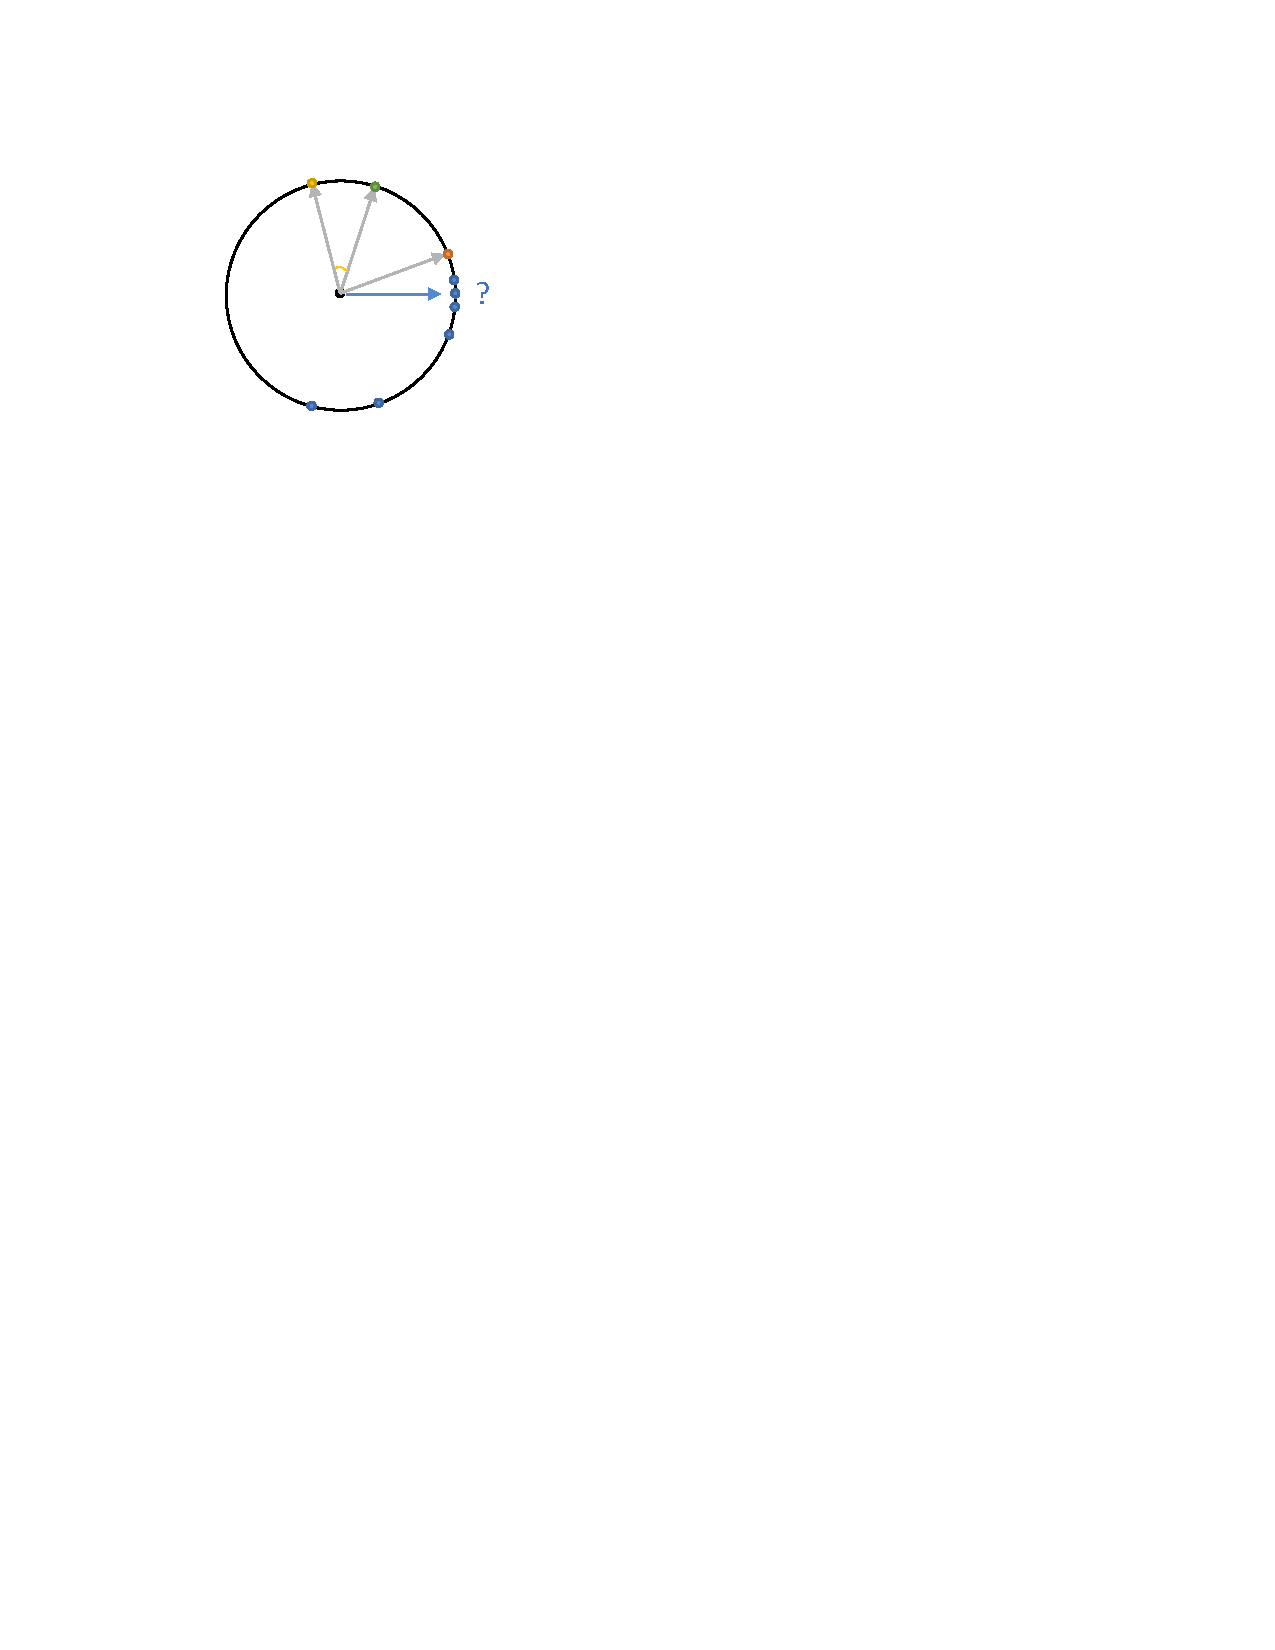
\includegraphics[width=0.25\linewidth]{meanshift1}
\label{a}}
\hfil
\subfloat[Shifting by the mean.]{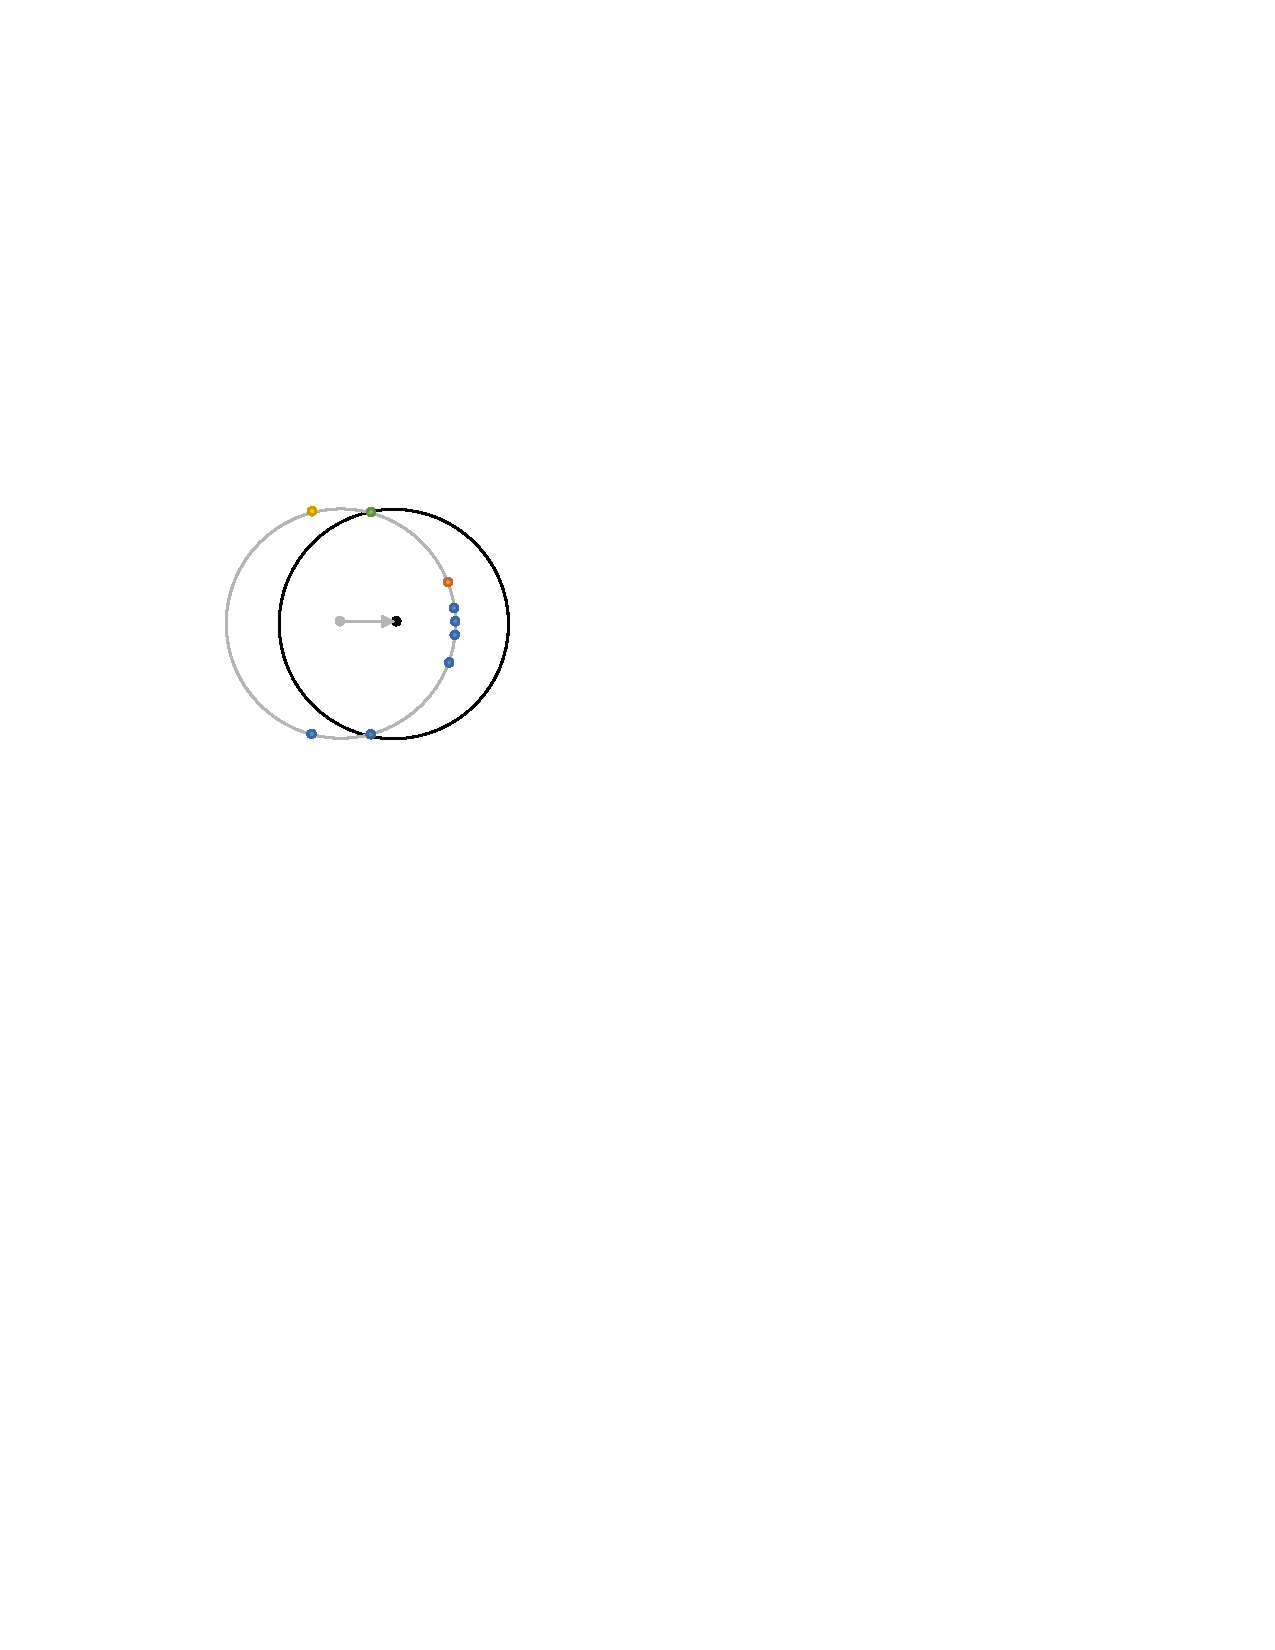
\includegraphics[width=0.25\linewidth]{meanshift2}%
\label{b}}
\hfil
\subfloat[Reprojecting on the unit sphere.]{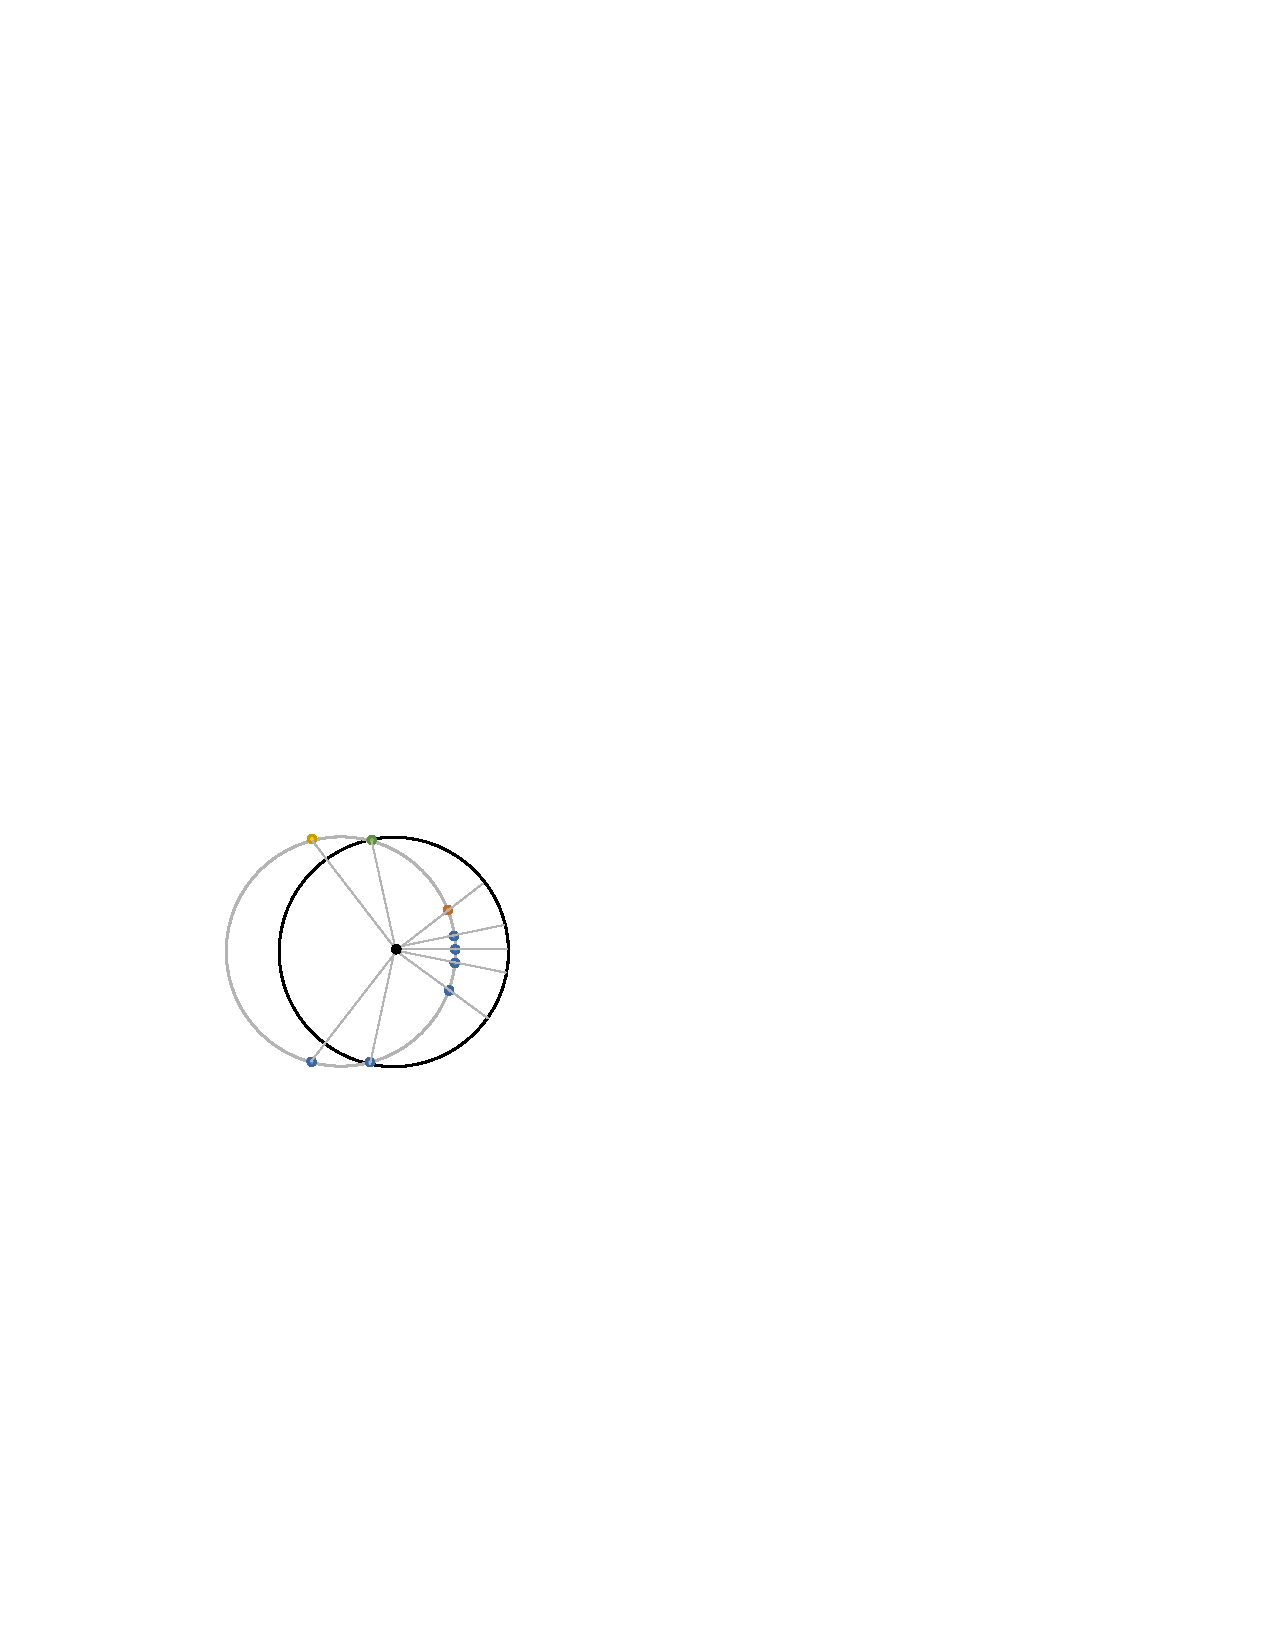
\includegraphics[width=0.25\linewidth]{meanshift3}%
\label{c}}
\hfil
\subfloat[Better discrimination of points]{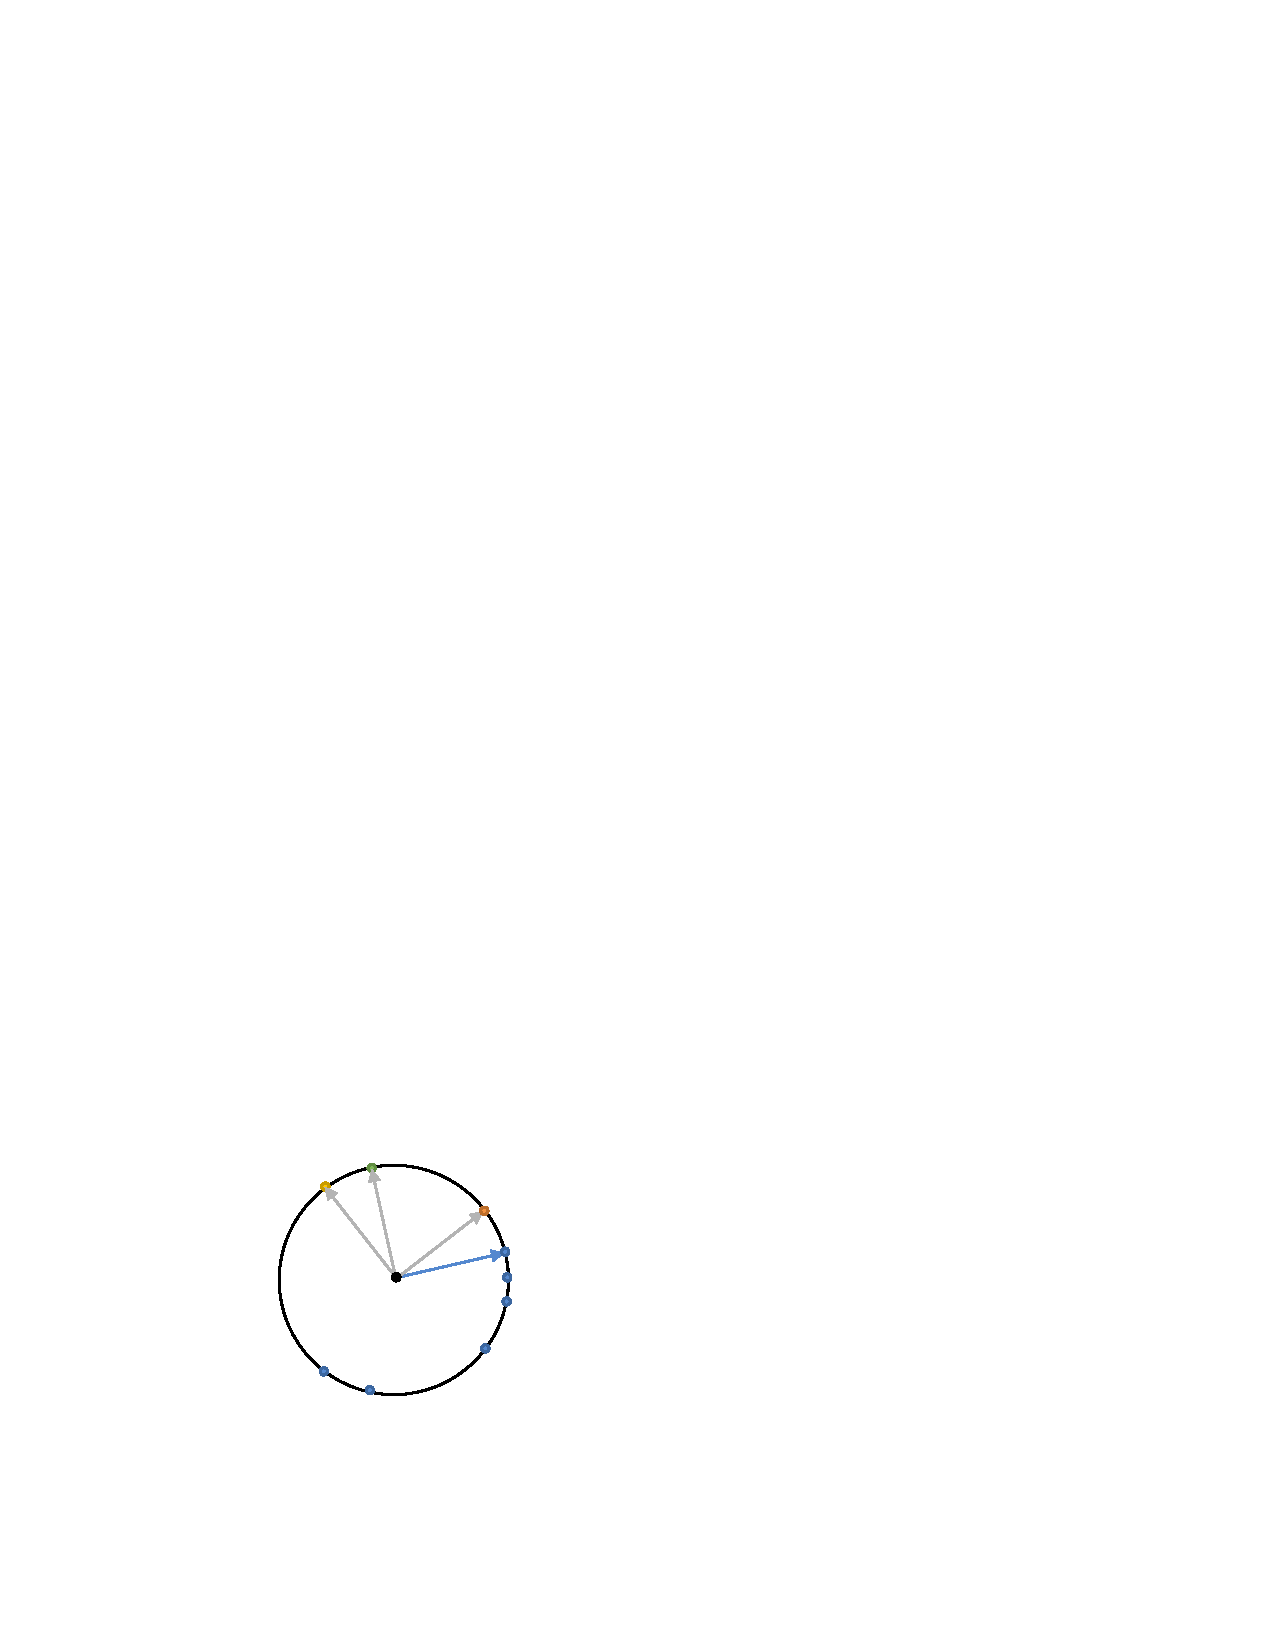
\includegraphics[width=0.22\linewidth]{meanshift4}%
\label{d}}
\caption{Sketch of the proposed mean-shift procedure in 2D. Consider the analogy "\textit{Yellow} is to \textit{Green} as \textit{Orange} is to ?". \textit{a)}: Unit sphere with projected vectors in respective colours. The points on the right are relatively close together and difficult to distinguish. \textit{b)}: The mean of all the points is computed and the centre of the sphere shifted. \textit{c)}: The re-projections of the points on the shifted sphere. \textit{d)}: The points are now farther apart and better distinguishable.}
\label{fig:ms}
\end{figure*}


\subsection{Mean-Shift for Better Discrimination}
\label{sec:ms}
Solving for the closest word in Equation \ref{eq:sim} based on the cosine similarity can be interpreted as projecting on an $N$-dimensional unit sphere and looking for the projected vector with smallest  angle to the given query vector. This projection can lead to similar vectors being very close on the sphere and therefore hard to distinguish based on angular distance. This observation is also backed up by the plots shown Figure \ref{fig:knn} where we observe that the correct word is often very close by. Being able to better distribute out the points on the sphere would therefore likely improve the predictions. 

We therefore propose the following mean-shift procedure:
\begin{enumerate}
\item Normalise all vectors (\textit{i.e.} project on the unit sphere)
\item Compute the mean of the normalised vectors
\item Shift by mean
\item Normalise again (\textit{i.e.} re-project on unit sphere)
\item Compute query vector with respect to the new normalised word vectors
\item Compute dot-products with query vector to get cosine-similarities
\end{enumerate}

The intuition behind this procedure is depicted in Figure \ref{fig:ms} which demonstrates how points very close by get distributed out. Note that the word arithmetic to compute the query vector is performed after the normalisation (otherwise no change in the results would be expected). We denote this approach with $CosMS$ in our experiments.


\subsection{Combining Analogy Interpretations}
We have already touched upon the idea that there are different ways of interpreting analogy exercises with respect to some similarity measure in Subsection \ref{sec:arithm}. The idea for Equation \ref{eq:anal2} for example is that we are looking for the vector $v$ most similar to $x$ and $u$ but dissimilar to $y$. We could however also pose it as looking for 
\begin{equation}
	v = \underset{v \in f(V)}{\text{argmin }}  |d(x, y)-d(u, v)|,
\end{equation}
that is $x$ and $y$ should have the same similarity as $u$ and $v$. Yet another option is to consider
\begin{equation}
	v = \underset{v \in f(V)}{\text{argmin }}  |d(x, u)-d(y, v)|.
\end{equation}
Note that these objectives all capture different aspects of the analogy, \textit{i.e.} they are not implying each other. We propose to combine these objectives in a weighted sum of these terms. Let $\phi$ denote the term in Equation \ref{eq:anal2}, \textit{i.e.}
\begin{equation}
	\phi(v)=d(v, u) - d(v, x) + d(v, y).
\end{equation}
We then want to maximise  the following expression:
\begin{equation}
	\phi(v) - \lambda \cdot (|d(x, y)-d(u, v)| +   |d(x, u)-d(y, v)|)
	\label{eq:alt}
\end{equation}
We set the weight parameter $\lambda = 0.1$ in our experiments and denote models using this similarity measure (including mean-shift) with $CosMS+$. 

\section{Experiments}
\label{sec:exp}

In this section we first outline our experimental setup, introduce novel test data
 and then report results obtained for different parameter choices and test scenarios. 

\subsection{Setup}
We used the Python re-implementation of word2vec contained in the Gensim library 
\cite{rehurek_lrec}. This implementation is functionally identical to the original 
C implementation provided by \cite{mikolov2013efficient}, but is easier to extend and has 
shown to perform just as well. 

To compare the influence of parameters on the performance we train several models
with different values for one of the parameters and keep all other parameters fixed. We 
identified the following set of parameters for our experiments:
\begin{enumerate}
\item Context-window size
\item Vector size (\textit{i.e.} dimension of hidden-layer)
\item Learning rate $\alpha$
\item Training corpus
\item Hierarchical softmax vs. negative sampling for Skip-Gram
\end{enumerate}

\subsection{Training Text Corpora}

We trained models using multiple text corpora to check if hyperparameters influence performance differently depending on the corpus.
These corpora include:
\subsubsection{Wiki}
The first 900 megabytes of the English Wikipedia dump on 03/03/2006.
\footnote{Instructions to download and build the test data on this website: http://mattmahoney.net/dc/textdata.html}

\subsubsection{Text8}
The first 100 megabytes of the English Wikipedia dump. Facilities for downloading and using this set are provided with word2vec.
\footnote{Ready-to-use corpus: http://mattmahoney.net/dc/text8.zip}

\subsubsection{Brown}
English corpus of one million words assembled from 500 sources of different genres, created in 1961 at Brown University.
It is considerably smaller than our other corpora.
We used this set and the sets below through the NLTK python library.
\footnote{See http://www.nltk.org/book/ch02.html}

\subsubsection{Treebank}
Fragment of the \textit{Penn Treebank} created in 1995 at the University of Pennsylvania. This contains material from the Wall Street Journal of 1989.

\subsubsection{Movie\_reviews}
Corpus of movie reviews up to 2004 from the website Rotten Tomatoes.

\subsection{New Test Data}
To test the models performance on domain-specific questions we constructed several 
questions sets. The questions are all of the form "X is to Y as U is to ?", \textit{i.e.} they take the 
form of analogies. We constructed the following sets of questions:

\subsubsection{Brand-Origin}
A set of questions testing for the relationship between well-known brands and their countries
of origin. To construct this questions set we gathered names and country of origin for 
the top 500 brands according to brandfinance.com. We excluded all the brands from countries
with names composed of multiple words (\textit{e.g.} United States of America, ...) due to the model 
working on single words. The result is a set of 38,220 questions.

\subsubsection{Movie-Director}
A set of analogy-questions for the relationship between famous movies and their respective 
directors. The set was constructed by gathering movie titles and last name of the director for 
some of the top rated movies according to IMDb. Similar to the Brand-Origin questions we 
excluded movies with titles composed of more than one word with the exception of titles
starting with "The ..." or similar.  The result is a set of 4,557 questions.


\section{Results}
\label{sec:res}

\begin{figure}[t]
\centering
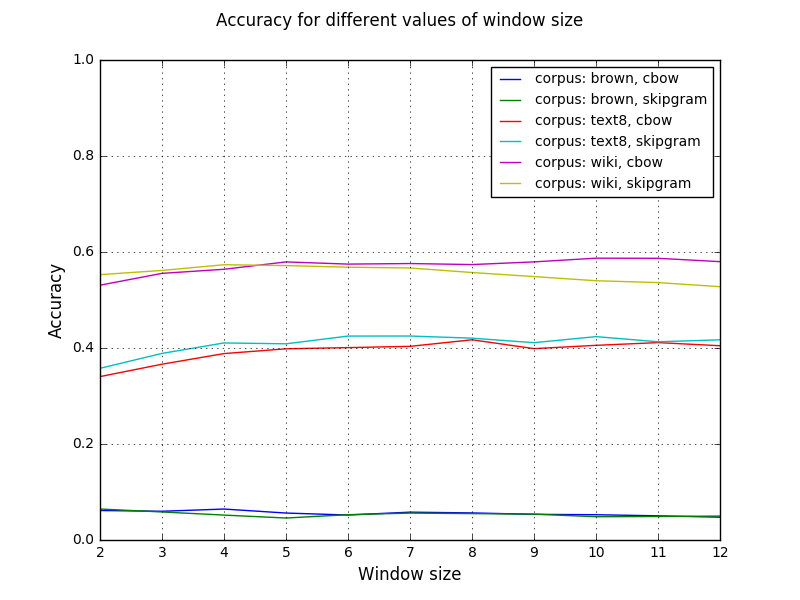
\includegraphics[width=0.5\textwidth]{graph_acc_window}
\caption{Accuracy for different values of the context-window size. }
\label{fig:window}
\end{figure}

\begin{figure}[t]
\centering
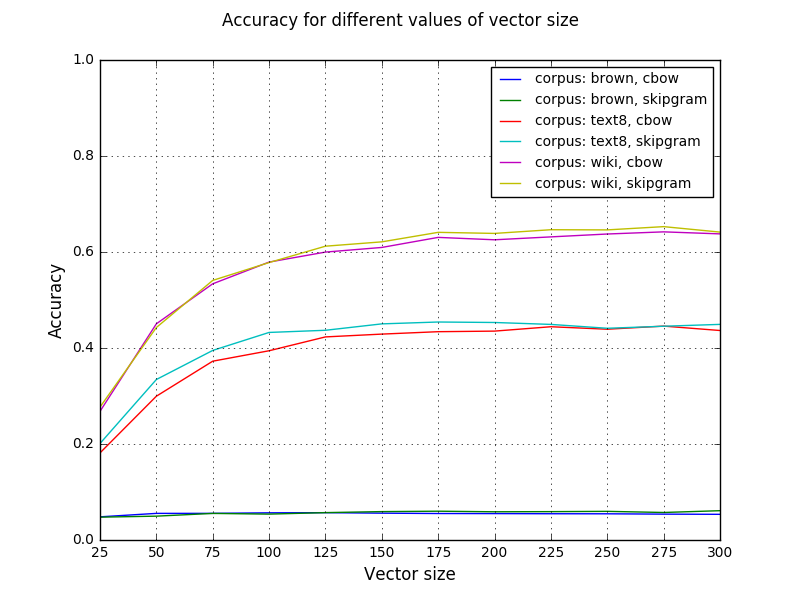
\includegraphics[width=0.5\textwidth]{graph_acc_size}
\caption{Accuracy for different values of vector-size (\textit{i.e.} dimension of embedding space). }
\label{fig:size}
\end{figure}

\begin{figure}[t]
\centering
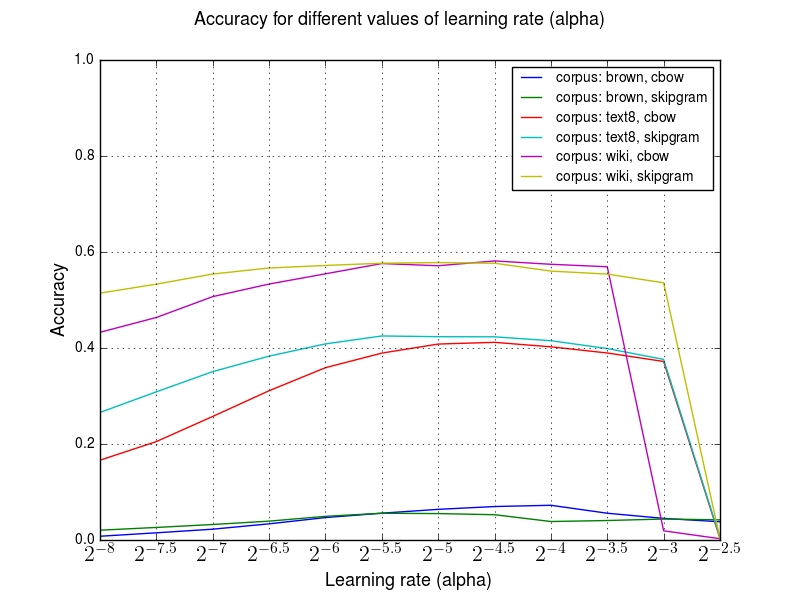
\includegraphics[width=0.5\textwidth]{graph_acc_alpha}
\caption{Accuracy for different values of the learning rate $\alpha$. }
\label{fig:alpha}
\end{figure}

\subsection{Influence of Parameters on Model Performance}
We first evaluate the influence of parameter choices using Google's generalised analogy dataset described in \cite{mikolov2013efficient}.
For this purpose we plotted the accuracy obtained for different values of a chosen parameter, while keeping all other parameters fixed. 
The baseline model for the comparison (with default parameter values) is shown in Table \ref{tab:baseline} .
Here, the accuracy is defined as the ratio of the number of right answers over the total number of questions.

\begin{table}[b]
\centering
\begin{tabular}{@{}c|c|c|c@{}}
\hline
\begin{tabular}[c]{@{}c@{}}Model- \\ Architecture \end{tabular} & \begin{tabular}[c]{@{}c@{}}Learning \\Rate $\alpha$\end{tabular}  & \begin{tabular}[c]{@{}c@{}}Window-\\ Size\end{tabular} & \begin{tabular}[c]{@{}c@{}}Vector-\\ Size\end{tabular} \\ \hline 
Skip-Gram &	0.025 	& 	5 	& 100	\\ \hline
\end{tabular}
\caption{The parameter values for the baseline model used in our experiments. }
\label{tab:baseline}
\end{table}

In Figure~\ref{fig:window} we see that the window size has only a limited influence on the accuracy.
It is also difficult to pinpoint a common best value but window sizes between 5 and 8 seem to work well on all corpora. 
Generally the model is quite robust with respect to this parameter.
Interestingly, a bigger window size seems beneficial when using CBOW on the wiki corpus, but detrimental when using Skip-Gram.

Conversely, we see in Figure~\ref{fig:size} that a large enough vector size is essential for good performance.
A larger value generally improves accuracy, although we get diminishing returns above a certain point.
This is not surprising as the vector size defines the complexity of the model and therefore also matters more for larger corpora.
Obviously the vector size also has some effect on training time, so it is wise to restrain the vector size.

The learning rate ($\alpha$) greatly affects performance as can be seen in Figure~\ref{fig:alpha}.
There appears to be a critical spot for $\alpha$ around which the accuracy drops dramatically (values around 0.03 - 0.15). 
However, a learning rate around 0.007 - 0.03 yields good results for every model we tried.
%TODO: I ignored the case "text8, cbow", I suspect there was an issue when drawing the graph.

From a broader perspective, we observe that the corpus size is by far what influences performance the most. This is not surprising given 
that neural networks are dependent on large amounts of training data. This is especially apparent when looking at the models trained on the $Brown$ corpus, which all fail to get reasonable accuracies.

Considering the choice of model architecture we also notice that  Skip-Gram slightly outperforms CBOW in most cases. It should be noted however that the Skip-Gram model is slightly more complex to train.


\begin{figure}[t]
\centering
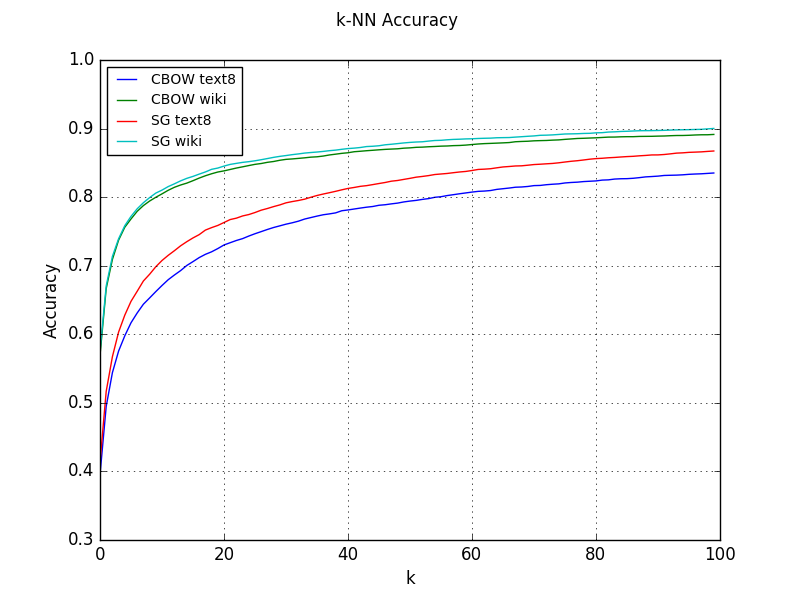
\includegraphics[width=0.5\textwidth]{graph_knn-acc}
\caption{k-NN accuracy according to k.}
\label{fig:knn}
\end{figure}

\subsection{K-NN Accuracy}
In cases when the model gives the wrong answer, the common definition of accuracy ignores how far off the model's prediction was from the correct answer. To get an idea of how wrong the model really is, we tried a different definition of accuracy where we consider the $k$ nearest neighbours of the prediction. We count the answer as a success if this set of neighbours contains the correct answer.

We plotted this k-NN accuracy for different values of \textit{k} in Figure~\ref{fig:knn}. It is clearly observable that the accuracy increases dramatically when changing from $k=1$ to $2$ or $3$ and only slowly starts saturating at around $k>10$. This suggests that the prediction is in fact not far off most of the time and suggests that small modifications to the similarity computations (such as the mean-shift) might have a positive effect on the performance. We also notice how models trained on larger corpora saturate faster and that the difference in performance between CBOW and Skip-Gram is more apparent in models trained on small corpora.
%TODO: Numbers guessed using the graph, may not be accurate

\begin{table*}[t]
\centering
\begin{tabular}{@{}c|cccc|cccccc|c@{}}
\hline
Method & \begin{tabular}[c]{@{}c@{}}Capital-\\Country\end{tabular} & \begin{tabular}[c]{@{}c@{}}Currency-\\Country\end{tabular} & \begin{tabular}[c]{@{}c@{}}City-\\State\end{tabular} & Family & \begin{tabular}[c]{@{}c@{}}Adjective-\\Adverb\end{tabular} & Opposite & Superlative &  \begin{tabular}[c]{@{}c@{}}Nationality-\\Adjective\end{tabular} & Past-tense & Plural & Total \\ \hline
$CosAdd$    & 47.4\%     &     21.3\%     &     22.2\%   &    63.7\%    &    15.1\%   &   15.4\%    &   40.1\%     &    77.8\%    &   32.9\%     &    48.3\%    &    43.0\%   \\
$Dice$      &    42.8\%     &    20.5\%      &    19.5\%    &    65.0\%    &   13.5\%     &     15.4\%  &    37.7\%    &    \textbf{79.2\%}    &    32.1\%    &     44.8\%   & 41.1\%        \\
$L^2$        &     44.0\%    &    14.9\%      &    20.6\%    &     60.1\%   &    15.2\%    &   11.8\%     &   27.7\%     &     74.9\%   &    30.2\%    &   42.8\%     &   39.9\%     \\
$L^1$ &    39.5\%     &     17.5\%     &     17.4\%   &    56.9\%    &    12.8\%    &   8.8\%     &   25.7\%     &    72.8\%    &   24.8\%     &    36.2\%    &    36.1\%   \\
$CosMul$   &        43.4\%    &    20.5\%     &    20.6\%   &     56.5\%   &    13.2\%    &   11.8\%     &   39.7\%    &     73.5\%   &    28.6\%   &   39.9\%   &   39.5\%     \\
$CosMS$   &        47.8\%    &    \textbf{21.6\%}      &    23.1\%   &     63.4\%   &    15.1\%    &   15.0\%     &   42.7\%    &     77.9\%   &    33.0\%    &   \textbf{49.3\%}    &   43.3\%     \\
$CosMS+$   &        \textbf{49.2\%}    &    21.3\%     &    \textbf{24.1\%}   &     \textbf{65.4\%}   &    \textbf{15.5\%}    &   \textbf{16.0\%}     &   \textbf{43.9\%}    &     78.4\%   &    \textbf{33.9\%}    &   47.7\%    &   \textbf{44.0\%}     \\
 \hline
\end{tabular}
\caption{Comparison of different similarity-measures. Results obtained on the generalised question set of \cite{mikolov2013efficient} with a Skip-Gram model trained on the \textit{Text8} corpus. We can observe that cosine-similarity overall performs better compared to the other measures.  Although not a similarity-measure by its own we list the results of our proposed mean-shift approach for comparison and note a slight increase in accuracy. Note that the total is computed as the micro-average (mean over all questions).} 
\label{tab:dists}
\end{table*}

\subsection{Similarity Measures}
To compare the different similarity measures introduced in Subsections \ref{sec:sim} and  \ref{sec:ms} we show results on selected categories of the generalised analogy dataset \cite{mikolov2013efficient} obtained with the baseline Skip-Gram model with parameters shown in Table \ref{tab:baseline}. 
The resulting accuracies are listed in Table \ref{tab:dists}. 

We observe that overall cosine similarities perform significantly better than the other similarity measures (with a few exceptions). Possible explanations for this circumstance are difficult to provide. For one we note that the Euclidean distance between weight-vectors are never explicitly used in the training of the model. In fact, the weight vectors only occur in dot-products with the columns of the hidden-to-out weight matrix $\boldsymbol{W'}$. Another explanation is that the norm of a word vector is related to the word-frequency as found by \cite{Schakel:2015aa} and is therefore not directly helpful in the analogy task.

\subsection{Mean Shift and Combination of Analogy Interpretations }
Tables \ref{tab:msWiki} and \ref{tab:mst8} show results comparing models with and without the proposed mean-shift and combination of analogy interpretations. Results for the models with mean-shift are indicated with \textit{CosMS}. We observe a slight overall improvement of models with mean-shift compared to the standard model for all the models. 

Models with the additional term of alternative analogy interpretations from Equation \ref{eq:alt} are depicted with \textit{CosMS+}. This has shown to further slightly improve the accuracy of the model.


\subsection{Domain Specific Questions}
TODO: S. Brulhart

Results for the domain specific questions will go here...

\begin{table}[]
	\centering
\begin{tabular}{c|cc|cc}
	\hline
	\multicolumn{1}{l|}{} & \multicolumn{2}{c|}{wiki} & \multicolumn{2}{c}{text8} \\ \cline{2-5} 
	\multicolumn{1}{l|}{\begin{tabular}[c]{@{}l@{}}Training\\ iterations\end{tabular}} & \begin{tabular}[c]{@{}c@{}}General\\ questions\end{tabular} & \begin{tabular}[c]{@{}c@{}}Specific\\ questions\end{tabular} & \begin{tabular}[c]{@{}c@{}}General\\ questions\end{tabular} & \begin{tabular}[c]{@{}c@{}}Specific\\ questions\end{tabular} \\ \hline
	0 & \textbf{57.80\%} & \textbf{9.62\%} & \textbf{43.28\%} & \textbf{5.65\%} \\
	1 & 50.72\% & 9.51\% & 36.97\% & 5.55\% \\
	2 & 40.43\% & 9.44\% & 31.84\% & 5.53\% \\
	3 & 37.11\% & 9.33\% & 28.50\% & 5.42\% \\
	10 & 30.21\% & 9.39\% & 22.45\% & 5.45\% \\ \hline
\end{tabular}
	\caption{Accuracy of models trained again with \textit{treebank} corpus against Brand-Origin questions}
	\label{tab:accu_treebank}
\end{table}


\begin{table}[]
	\centering
\begin{tabular}{c|cc|cc}
	\hline
	\multicolumn{1}{l|}{} & \multicolumn{2}{c|}{wiki} & \multicolumn{2}{c}{text8} \\ \cline{2-5} 
	\multicolumn{1}{l|}{\begin{tabular}[c]{@{}l@{}}Training\\ iterations\end{tabular}} & \begin{tabular}[c]{@{}c@{}}General\\ questions\end{tabular} & \begin{tabular}[c]{@{}c@{}}Specific\\ questions\end{tabular} & \begin{tabular}[c]{@{}c@{}}General\\ questions\end{tabular} & \begin{tabular}[c]{@{}c@{}}Specific\\ questions\end{tabular} \\ \hline
	0 & \textbf{57.80\%} & \textbf{2.32\%} & \textbf{43.27\%} & 1.18\% \\
	1 & 32.96\% & 1.52\% & 24.75\% & \textbf{2.26\%} \\
	2 & 20.15\% & 1.07\% & 14.97\% & 1.51\% \\
	3 & 14.42\% & 0.89\% & 11.26\% & 1.40\% \\
	10 & 6.28\% & 0.80\% & 5.28\% & 0.54\% \\ \hline
\end{tabular}
	\caption{Accuracy of models trained again with \textit{movie\_reviews} corpus against Movie-Director questions}
	\label{tab:accu_movie_reviews}
\end{table}

\begin{table*}[t]
\centering
\begin{tabular}{@{}c|cccc|cccccc|c@{}}
\hline
Model & \begin{tabular}[c]{@{}c@{}}Capital\\Country\end{tabular} & \begin{tabular}[c]{@{}c@{}}Currency\\Country\end{tabular} & \begin{tabular}[c]{@{}c@{}}City\\State\end{tabular} & Family & \begin{tabular}[c]{@{}c@{}}Adjective\\Adverb\end{tabular} & Opposite & Superlative &  \begin{tabular}[c]{@{}c@{}}Nationality\\Adjective\end{tabular} & Past-tense & Plural & Total \\ \hline
CBOW  & 63.6\%  & 19.1\%   & 42.8\% & \textbf{79.7\%} & 28.4\% & 36.0\% & 62.3\% & 84.3\% & 45.3\% & 67.8\% & 58.7\% \\
CBOW $CosMS$    &    63.9\%     &    19.7\%      &    43.9\%    &    \textbf{79.7\%}    &   28.4\%     &    35.7\%  &    \textbf{63.4\%}    &    83.9\%   &    45.3\%    &     67.8\%   & 59.1\%        \\
CBOW $CosMS+$    &    64.9\%     &    20.2\%      &    \textbf{44.5\%}    &    79.2\%    &   28.8\%     &    34.2\%  &    \textbf{63.4\%}    &    83.7\%   &    44.4\%    &     67.8\%   & 59.1\%        \\

Skip-Gram &    70.4\%     &     21.3\%     &     34.6\%   &    70.5\%    &    \textbf{29.2\%}    &   \textbf{38.6\%}     &   58.7\%     &    89.4\%    &   49.2\%     &    69.3\%    &    59.2\%   \\
Skip-Gram $CosMS$  &     70.5\%   &    21.3\%      &    35.9\%   &     70.8\%   &    28.3\%    &   \textbf{38.6\%}     &   58.7\%    &     \textbf{89.5\%}   &    \textbf{49.6\%}    &   70.0\%    &   59.4\%     \\
Skip-Gram $CosMS+$  &     \textbf{71.6\%}    &    \textbf{21.9\%}      &    37.4\%   &     73.7\%   &    28.0\%    &   37.7\%     &   60.1\%    &     88.9\%   &    48.6\%    &   \textbf{70.1\%}    &   \textbf{60.0\%}     \\

 \hline
\end{tabular}
\caption{Performance comparison of models with and without our proposed mean-shift approach. Results obtained on the generalised question set of \cite{mikolov2013efficient} with models trained on the \textit{Wiki} corpus.}
\label{tab:msWiki}
\end{table*}

\begin{table*}[t]
\centering
\label{my-label}
\begin{tabular}{@{}c|cccc|cccccc|c@{}}
\hline
Model & \begin{tabular}[c]{@{}c@{}}Capital\\Country\end{tabular} & \begin{tabular}[c]{@{}c@{}}Currency\\Country\end{tabular} & \begin{tabular}[c]{@{}c@{}}City\\State\end{tabular} & Family & \begin{tabular}[c]{@{}c@{}}Adjective\\Adverb\end{tabular} & Opposite & Superlative &  \begin{tabular}[c]{@{}c@{}}Nationality\\Adjective\end{tabular} & Past-tense & Plural & Total \\ \hline
CBOW  & 33.5\%  & 16.4\%   & 14.7\% & \textbf{79.7\%} & 13.9\% & \textbf{20.3\%} & 42.3\% & 65.4\% & 30.3\% & 44.7\% & 39.5\% \\
CBOW $CosMS$   &    35.3\%     &    17.5\%      &    15.8\%    &    78.4\%    &   14.9\%     &    19.9\%  &    42.3\%   &    64.9\%   &    31.0\%    &     45.3\%   & 39.8\%        \\
CBOW $CosMS+$   &    35.5\%     &    16.4\%      &    16.3\%    &    79.4\%    &   14.4\%     &    19.0\%  &    44.1\%   &    64.9\%   &    30.3\%    &     46.1\%   & 40.0\%        \\
Skip-Gram &    47.4\%     &     21.3\%     &     22.2\%   &    63.7\%    &    15.1\%    &   15.4\%     &   40.1\%     &    77.8\%    &   32.9\%     &    48.3\%    &    43.0\%   \\
Skip-Gram+RC  &     47.8\%    &    \textbf{21.6\%}      &    23.1\%   &     63.4\%   &    15.1\%     &   15.0\%     &   42.7\%    &     77.9\%   &    33.0\%    &   \textbf{49.3\%}    &   43.3\%    \\
Skip-Gram $CosMS+$   &        \textbf{49.2\%}    &    21.3\%     &    \textbf{24.1\%}   &     65.4\%   &    \textbf{15.5\%}    &   16.0\%   &   \textbf{43.9\%}    &     \textbf{78.4\%}   &    \textbf{33.9\%}    &   47.7\%    &   \textbf{44.0\%}     \\
 \hline
\end{tabular}
\caption{Performance comparison of models with and without our proposed mean-shift approach. Results obtained on the generalised question set of \cite{mikolov2013efficient} with models trained on the \textit{Text8} corpus.}
\label{tab:mst8}
\end{table*}




\section{Discussion}

\subsection{Limitations}
TODO: S. Brulhart



\subsection{Future Work}
TODO: S. Brulhart


\subsection{Conclusion}

In this work we studied the influence of several parameter choices on the performance of word2vec models.
We found that the learning rate $\alpha$, the size of the hidden layer and the choice of architecture are critical while the window size has not shown to affect the performance significantly. Not surprisingly however, the size of the training corpus has shown to be the most important factor on the performance of the model. By analysing the k-NN accuracy we observed that the model's guesses are usually very close to the correct answer.

In a comparison of different similarity measures we verified the superiority of the cosine similarity over other alternatives. We proposed to use mean-shift and a combination of analogy interpretations and showed how they lead to improvements in accuracy.

\label{sec:end}



% An example of a floating figure using the graphicx package.
% Note that \label must occur AFTER (or within) \caption.
% For figures, \caption should occur after the \includegraphics.
% Note that IEEEtran v1.7 and later has special internal code that
% is designed to preserve the operation of \label within \caption
% even when the captionsoff option is in effect. However, because
% of issues like this, it may be the safest practice to put all your
% \label just after \caption rather than within \caption{}.
%
% Reminder: the "draftcls" or "draftclsnofoot", not "draft", class
% option should be used if it is desired that the figures are to be
% displayed while in draft mode.
%
%\begin{figure}[!t]
%\centering
%\includegraphics[width=2.5in]{myfigure}
% where an .eps filename suffix will be assumed under latex,
% and a .pdf suffix will be assumed for pdflatex; or what has been declared
% via \DeclareGraphicsExtensions.
%\caption{Simulation results for the network.}
%\label{fig_sim}
%\end{figure}

% Note that the IEEE typically puts floats only at the top, even when this
% results in a large percentage of a column being occupied by floats.


% An example of a double column floating figure using two subfigures.
% (The subfig.sty package must be loaded for this to work.)
% The subfigure \label commands are set within each subfloat command,
% and the \label for the overall figure must come after \caption.
% \hfil is used as a separator to get equal spacing.
% Watch out that the combined width of all the subfigures on a
% line do not exceed the text width or a line break will occur.
%
%\begin{figure*}[!t]
%\centering
%\subfloat[Case I]{\includegraphics[width=2.5in]{box}%
%\label{fig_first_case}}
%\hfil
%\subfloat[Case II]{\includegraphics[width=2.5in]{box}%
%\label{fig_second_case}}
%\caption{Simulation results for the network.}
%\label{fig_sim}
%\end{figure*}
%
% Note that often IEEE papers with subfigures do not employ subfigure
% captions (using the optional argument to \subfloat[]), but instead will
% reference/describe all of them (a), (b), etc., within the main caption.
% Be aware that for subfig.sty to generate the (a), (b), etc., subfigure
% labels, the optional argument to \subfloat must be present. If a
% subcaption is not desired, just leave its contents blank,
% e.g., \subfloat[].


% An example of a floating table. Note that, for IEEE style tables, the
% \caption command should come BEFORE the table and, given that table
% captions serve much like titles, are usually capitalized except for words
% such as a, an, and, as, at, but, by, for, in, nor, of, on, or, the, to
% and up, which are usually not capitalized unless they are the first or
% last word of the caption. Table text will default to \footnotesize as
% the IEEE normally uses this smaller font for tables.
% The \label must come after \caption as always.
%
%\begin{table}[!t]
%% increase table row spacing, adjust to taste
%\renewcommand{\arraystretch}{1.3}
% if using array.sty, it might be a good idea to tweak the value of
% \extrarowheight as needed to properly center the text within the cells
%\caption{An Example of a Table}
%\label{table_example}
%\centering
%% Some packages, such as MDW tools, offer better commands for making tables
%% than the plain LaTeX2e tabular which is used here.
%\begin{tabular}{|c||c|}
%\hline
%One & Two\\
%\hline
%Three & Four\\
%\hline
%\end{tabular}
%\end{table}


% Note that the IEEE does not put floats in the very first column
% - or typically anywhere on the first page for that matter. Also,
% in-text middle ("here") positioning is typically not used, but it
% is allowed and encouraged for Computer Society conferences (but
% not Computer Society journals). Most IEEE journals/conferences use
% top floats exclusively.
% Note that, LaTeX2e, unlike IEEE journals/conferences, places
% footnotes above bottom floats. This can be corrected via the
% \fnbelowfloat command of the stfloats package.


% conference papers do not normally have an appendix



% trigger a \newpage just before the given reference
% number - used to balance the columns on the last page
% adjust value as needed - may need to be readjusted if
% the document is modified later
%\IEEEtriggeratref{8}
% The "triggered" command can be changed if desired:
%\IEEEtriggercmd{\enlargethispage{-5in}}

% references section

% can use a bibliography generated by BibTeX as a .bbl file
% BibTeX documentation can be easily obtained at:
% http://mirror.ctan.org/biblio/bibtex/contrib/doc/
% The IEEEtran BibTeX style support page is at:
% http://www.michaelshell.org/tex/ieeetran/bibtex/
\bibliographystyle{IEEEtran}
% argument is your BibTeX string definitions and bibliography database(s)
\bibliography{IEEEabrv,./bibliography}




% that's all folks
\end{document}
